\chapter{Beam Spin Asymmetry Analysis}

\section{Introduction}
Measurement of the beam spin asymmetry is carried out for the positively charged K-meson.  As discussed in the introduction, the beam spin asymmetry theoretically depends on $F_{UU,L}$, $F_{UU,T}$, $F_{UU}^{\cos\phi}$, $F_{UU}^{\cos 2\phi}$, and $F_{LU}^{\sin\phi}$.  By dividing the electron-kaon events into several bins, beam spin asymmetry measurements are taken at different average values of the kinematic variables $x$, $Q^2$, $z_h$, and $P_T$.  Finally, the structure function ratios $A_{LU}^{\sin\phi}$, $A_{UU}^{\cos\phi}$, and $A_{UU}^{\cos 2\phi}$ are extracted from each bin.  In this chapter a discussion is provided of SIDIS event selection, the binning used in this analysis, measurement values with associated systematic uncertainties, and the extraction of structure function ratios using the $\phi_h$ dependence in each kinematic bin.

\section{Event Selection and Binning}
\subsubsection*{Event Selection}
After particle identification, events which have a trigger electron and a positive kaon are kept for analysis.  Events are discarded that do not have $W > 2 \; GeV/c^2$ and $Q^2 > 1 \; GeV^2/c^2$, because they are not considered part of the deeply inelastic region.  Additionally, to avoid exclusive resonances in the $ep \rightarrow eK^+X$ spectrum, a minimum value is imposed on the missing mass of the final state $M_X$ ($ep \rightarrow eK^+X$).  Here, we use $M_{X} (ep \rightarrow eK^+X) > 1.25 \; GeV/c^2$.  Finally, a cut is applied to exclude low values of $z$ to constrain our kinematics to the current factorization region where TMD factorization has been demonstrated at leading order.  It is additionally required that $z < 0.75$ to avoid exclusive events.  This restriction on $z$ is applied when $z$ is integrated over (for the axes $x$, $Q^2$, and $P_T$) but not to the $z$ axis itself, where we measure the asymmetry across the entire experimentally observed kinematic range.  

\easyFigure{image/plots/kaon-bsa/z-pt2.pdf}{Correlation between $z$ and $P_{T}^{2} \; (GeV^2/c^2)$ for each event in our analysis sample.} 

% I'm not sure where to put this figure. 
\begin{figure}
	\centering
	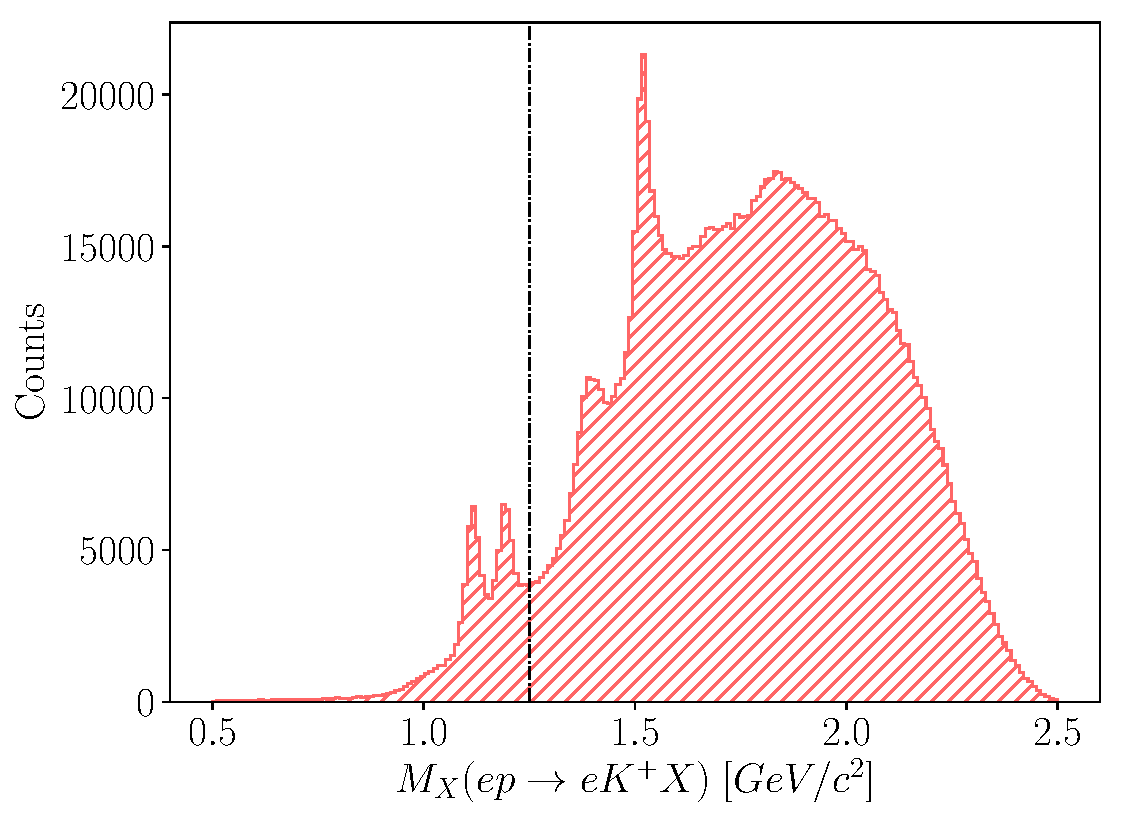
\includegraphics[width=16cm]{image/plots/kaon-bsa/mx.pdf}
	\caption{The missing mass spectrum for the reaction $ep \rightarrow e'K^+X$ is shown after the application of all cuts used in the analyses except for the cut we apply on the missing mass.}
\end{figure}

\subsubsection*{Binning}

% This is the ugliest figure in the history of physics.
%\easyFigure{image/plots/kaon-bsa/binning.pdf}{The binning used for each of the kinematic axes.}
The beam spin asymmetry measurement is performed for the kinematic variables $x$, $Q^2$, $z$, and $P_T$.  For each variable 5 bins are chosen, as well as 12 bins in $\phi$ for a total of 60 analysis bins. \\

Bins were chosen using a simple method to ensure equal statistics in each kinematic variable bin (the phi bins do not have equal statistics).  The procedure is described using the axis $x$ as an example.  First, all events are sorted by their $x$ value from smallest to largest.  Then, the smallest and largest values are recorded, which are $x_1$ and $x_N$ if there are N events in the sample.  Next, the target number of bins M is chosen (this choice depends on each analysis).  Finally, the limits of each bin can be chosen by calculating the number of events per bin $N/M$ and then using the value of $x$ which corresponds to multiples of $N/M$ in the sample.    

\begin{equation}
  \vec{b} = (x_1, x_{N/M}, x_{2N/M}, ..., x_N)
\end{equation}

Here, the symbol $\vec{b}$ denotes a vector of (M+1) $x$ values which represent bin limits.  The binning in $\phi$ is chosen to be regularly spaced between -180 and 180 degrees.    

\begin{figure}
	\centering
	\label{fig:binning-z-phi}
	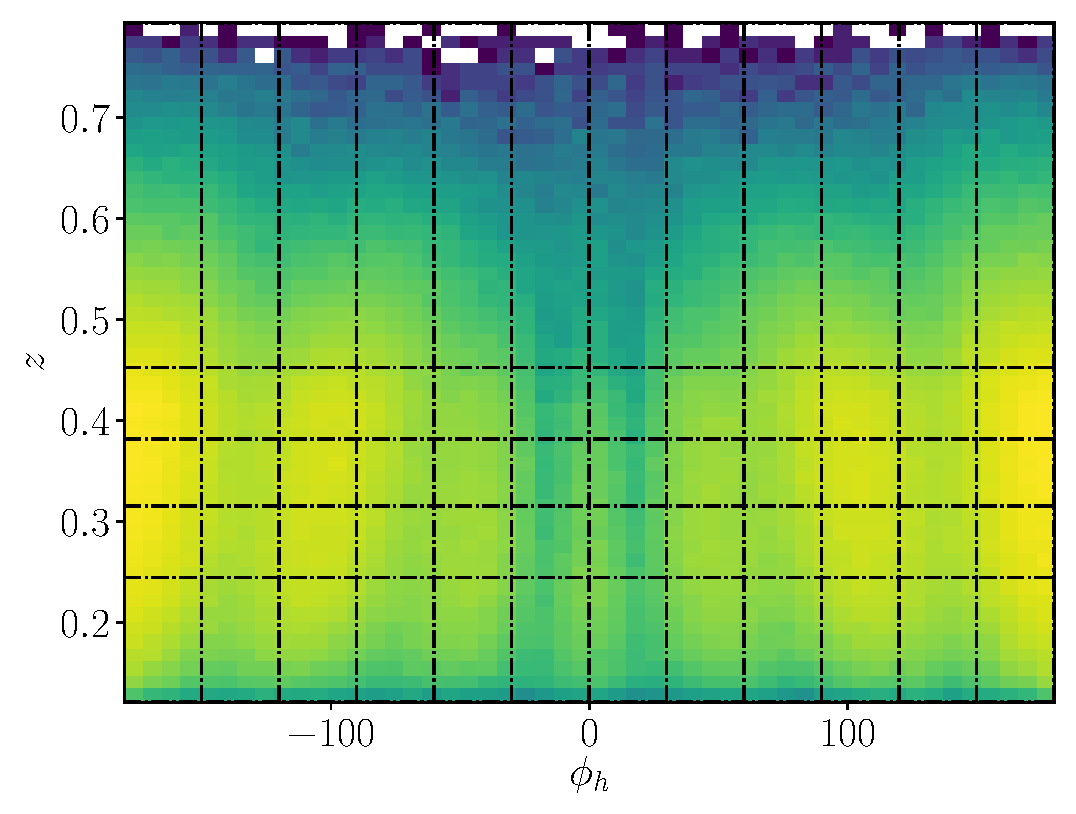
\includegraphics[width = 12cm]{image/plots/kaon-bsa/binning_z_phi.pdf}
	\caption{Bins used for this analysis are displayed in two dimensions for the $z$ axis.}
\end{figure}

\section{Measured $\phi_h$ Distributions}
\subsection*{Measured Asymmetry Values}
In each bin $i$ the beam spin asymmetry (here $A_i$) is calculated according to, 

\begin{equation}
  A_i = \frac{1}{P_e} \frac{n_+^i - n_-^i}{n_+^i + n_-^i}
\end{equation}

where $P_e$ is the average beam polarization over the dataset (74.9\%).  The symbols $n_{\pm}^{i}$ refer to the number of events counted in bin $i$ with helicity $\pm$.  

\begin{equation}
	\centering
	\label{fig:bsa-sys-x}
	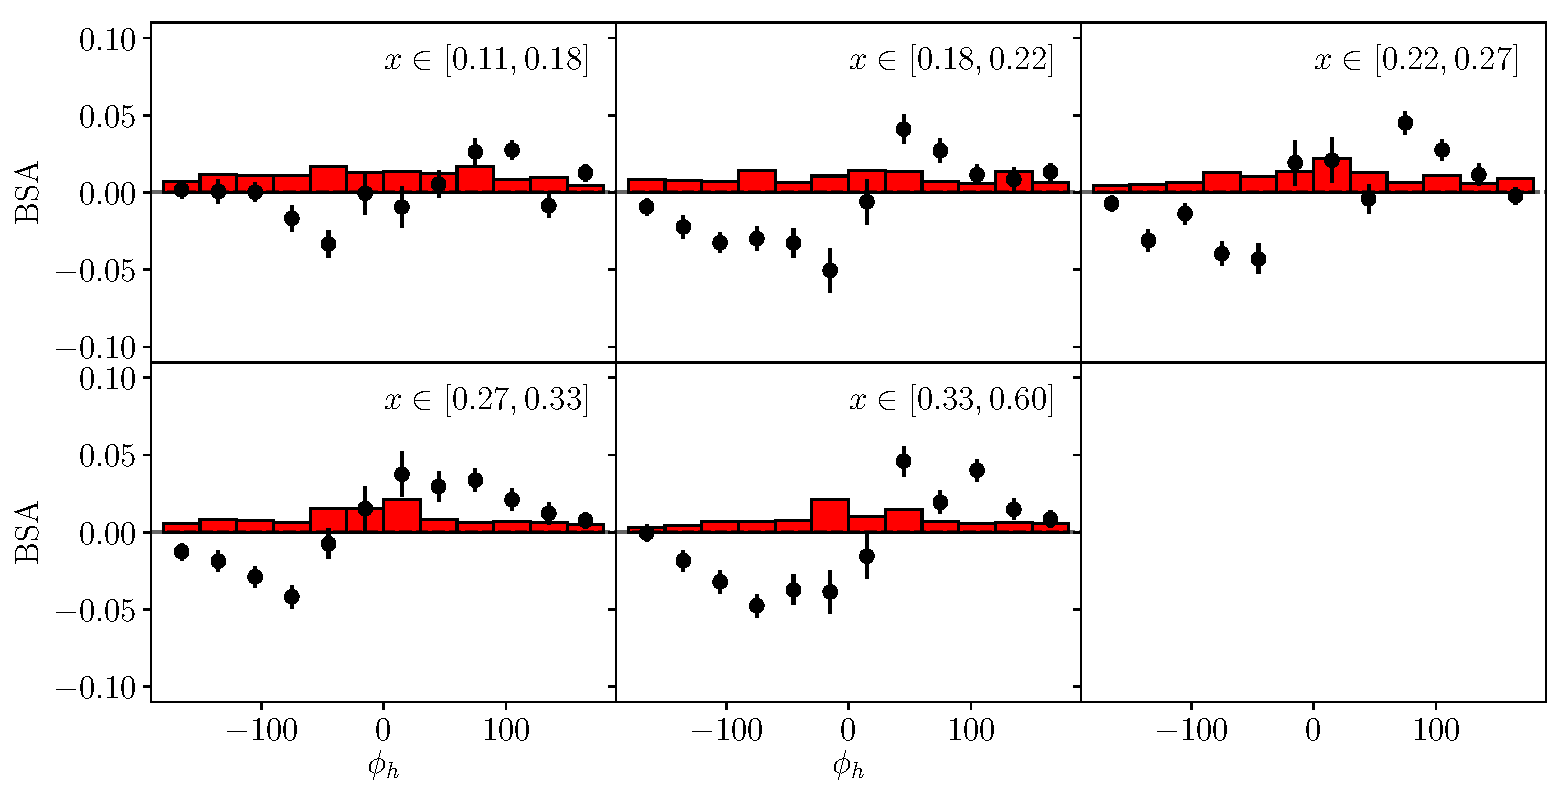
\includegraphics[width=\textwidth]{image/plots/kaon-bsa/grid_bsa_sys_x.pdf}
	\caption{The $\phi_h$ dependence is shown for each bin of $x$, increasing in value from the top left to the bottom right.  The statistical uncertainty is shown as black error bars on each point.  The total systematic uncertainty is shown as a red bar centered at zero.}
\end{equation}

\begin{equation}
	\centering
	\label{fig:bsa-sys-z}
	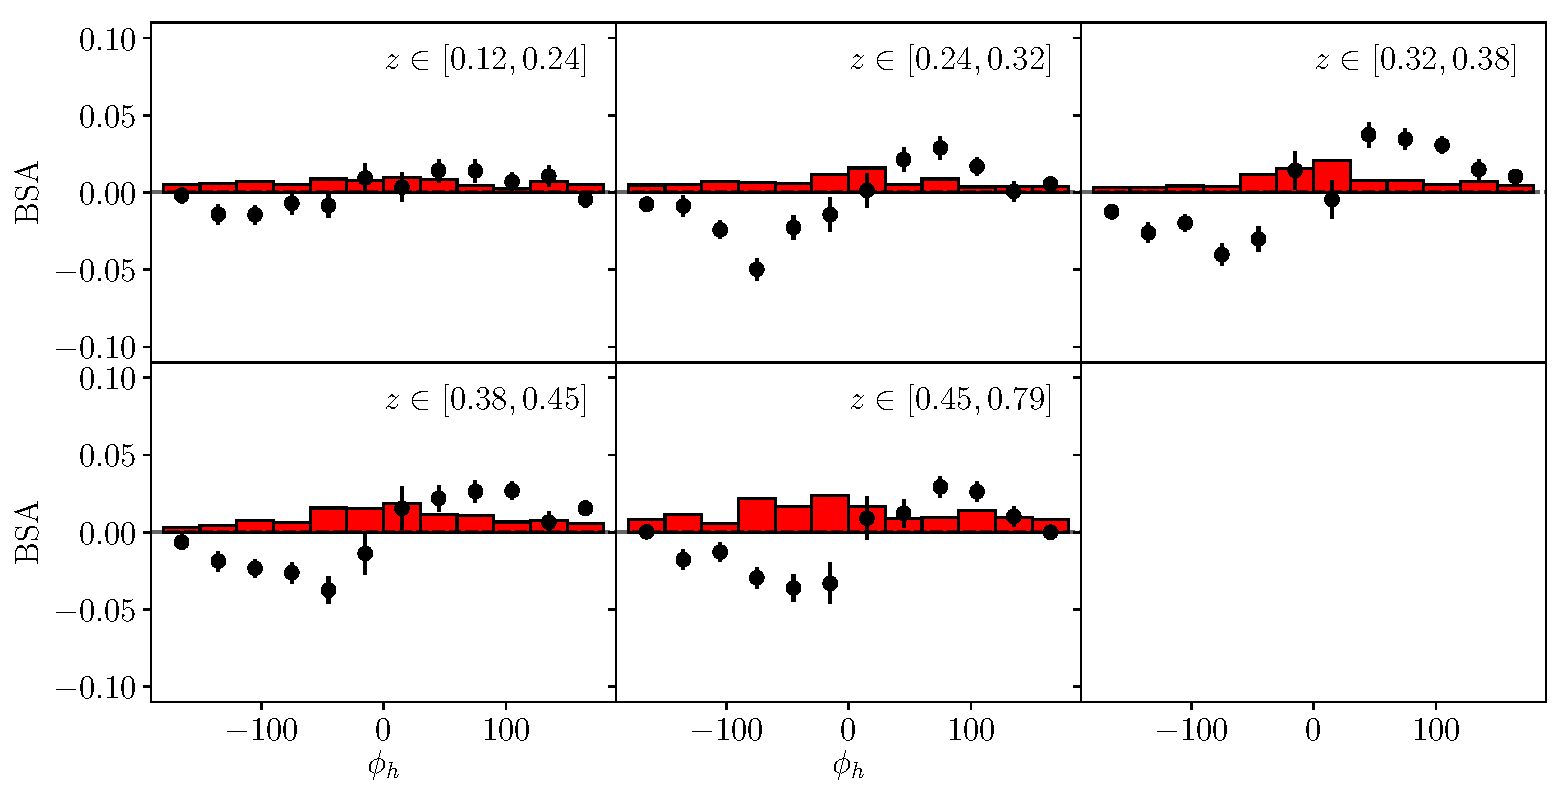
\includegraphics[width=\textwidth]{image/plots/kaon-bsa/grid_bsa_sys_z.pdf}
	\caption{The $\phi_h$ dependence is shown for each bin of $z$, increasing in value from the top left to the bottom right.  The statistical uncertainty is shown as black error bars on each point.  The total systematic uncertainty is shown as a red bar centered at zero.}
\end{equation}

\subsection*{Statistical Uncertainties}
The uncertainty on the measured value of $A_i$ can be attributed to statistical uncertainty on the counts $n_{i}^{\pm}$, and the uncertainty associated with the measurement of $P_e$.  The statistical uncertainty reported on the measurement includes the contribution from counts, but not from the uncertainty in $P_e$ which is included in the systematic errors.  In general, the uncertainty in a measured observable $\mathcal{O}$ depends on the uncertainty of the parameters (here denoted by $\vec{\theta}$) used in the analysis in the following way (see appendix for derivation).

\begin{equation}
  \label{eqn:error-propagation}
  \sigma_{\mathcal{O}}^2 = \sum_{i=1}^{N} \sum_{j=1}^{N} \frac{\partial \mathcal{O}}{\partial \theta_i} \frac{\partial \mathcal{O}}{\partial \theta_j} \rho_{ij} \sigma_i \sigma_j 
\end{equation}
  
For the beam spin asymmetry in the $i^{th}$ bin $A_i$ one finds that without correlations ($\rho_{ij} = \delta_{ij}$) the error propagation proceeds as shown below.

\begin{equation}
  \sigma_{A}^{2} = \frac{A^2}{P_{e}^2} \sigma_{P_{e}}^{2} + \frac{4 (n_{-}^{2} \sigma_{+}^{2}  + n_{+}^{2} \sigma_{-}^{2})}{ P_{e}^{2} (n_{+} + n_{-})^4}
\end{equation} 

The first term which is the contribution from the variance in the measurements of beam polarization will be included as a systematic error.  The second term is used as the statistical error bars shown through the analysis.  The counts $n_{\pm}^{i}$ for the $i^{th}$ bin are assumed to be Poisson in nature, and therefore have a variance equal to the expected number of counts $\sigma_{\pm}^{2} = n_{\pm}^{i}$.  With this expression for the statistical uncertainty on the counts, and dropping the beam polarization term for now, the expression becomes: 

\begin{equation}
  \sigma_{A}^{2} = \frac{4n_+ n_-}{P_{e}^{2} (n_+ + n_-)^3}
\end{equation}

\subsection*{Systematic Uncertainties}

% ---------------------------------------
%   Here is a general description of 
%   the treatment of systematics. 
% ---------------------------------------

\subsubsection*{Basic Formalism}

Systematic effects are shifts or biases in the measured result of some observable as a result of the procedure used in the measurement.  Systematic effects can typically be identified and corrected for, or removed all together from the measurement.  In the cases where an effect cannot be completely removed, the degree to which the correction for the effect is uncertain is included in the result of the measurement as a systematic uncertainty \cite{misc-barlow:2002}. \\

\easyFigure{image/diagrams/linear-error.pdf}{The analysis is run for variations in the input parameters $\theta_i$ to calculate the dependence of the result $\mathcal{O}$ on each parameter, as described in this section.}

Systematic uncertainties are included using the standard equation for error propagation.  In some cases it is possible to analytically find the derivatives needed to calculate the dependence of the observable on a source of systematic uncertainty.  This is the case for effect of the variance of the beam polarization on the beam spin asymmetry observable.  However in many cases, it is not possible to analytically calculate the effect of an analysis parameter $\theta_i$ on the observable $\mathcal{O}$.  Since the observable is usually calculated using some computational chain which starts with the input parameters $\vec{\theta}$, it is possible to find the dependence of the observable $\mathcal{O}$ on the inputs numerically.

\begin{equation}
  \frac{\partial \mathcal{O}}{ \partial \theta_i} \approx \frac{\mathcal{O}(\theta_i + \sigma_{\theta_i}/2) - \mathcal{O}(\theta_i - \sigma_{\theta_i}/2)}{\sigma_{\theta_i}}
\end{equation}

After inserting the above into equation \ref{eqn:error-propagation} one finds,

\begin{equation}
  \sigma_{\mathcal{O}}^{2} = \sum_{i=1}^{n} \sum_{j=1}^{n} \rho_{ij} (\mathcal{O}(\theta_i + \sigma_{\theta_i}/2) - \mathcal{O}(\theta_i - \sigma_{\theta_i}/2)) (\mathcal{O}(\theta_j + \sigma_{\theta_j}/2) - \mathcal{O}(\theta_j - \sigma_{\theta_j}/2)) 
\end{equation}

where $\rho_{ij}$ is the correlation $V_{ij}/\sigma_i \sigma_j$.  In most cases, these correlations are assumed to be zero.  In some cases, when the parameters $\theta_i$, $\theta_j$ come from a fit one may have a correlation provided by the covariance matrix and it should be used.  In the case where correlations are assumed to be zero, the total systematic uncertainty is simply the quadratic sum of the shifts in the observable within the uncertainty window on each parameter.

\begin{equation}
  \sigma_{\mathcal{O}}^{2} = \sum_{i=1}^{n} \Bigl[ \mathcal{O}(\theta_i + \sigma_{\theta_i}/2) - \mathcal{O}(\theta_i - \sigma_{\theta_i}/2) \Bigr]^2
\end{equation}

\subsubsection*{Sources of Systematic Uncertainty}
Systematic uncertainties are calculated using the techniques described above for both the $\phi_h$ dependent asymmetry measurement as well as the results of the parameter estimation for each kinematic bin.  The systematic errors on the phi dependent asymmetry bins is not used in the parameter estimation for the structure function ratios $A$.  Table \ref{table:kaon-systematics} below summarizes the sources of systematic uncertainty considered in this analysis.

% --------------------
%    table of sys 
% --------------------
\begin{table}
  \centering
  \begin{tabular}{c|c|c}
    Source                     & Variation  \\ 
    \hline
    Beam polarization                  & 0.024        \\ 
    DC Region 1 Fid.                     & 1 (cm)         \\ 
    DC Region 3 Fid.                    & 3 (cm)        \\
    EC-W                                       & 12 (cm)         \\ 
    EC-V                                        & 12 (cm)        \\
    EC-U                                        & 12 (cm)        \\
    Kaon Confidence ($\alpha$) & 0.5-0.6     \\
    $\theta_{cc}$ Matching         & $\sigma$        \\
    EC Energy Deposition            & 0.01 (GeV)      \\
    $p_{K^+}$                               & 1.9-2.1  \\ 
    EC Sampling Fraction             & $0.5 \sigma$    \\
    Z-Vertex                                  & 0.5 (cm)        \\
    Vertex diff.                              & 1 (cm)  \\
    \hline 
  \end{tabular}
  \caption{Different sources of systematic effect considered in this analysis.  The magnitude of the effect is shown here averaged over all bins of $\phi_h$.}
  \label{table:kaon-systematics}
\end{table}

Except for the beam polarization and the momentum of the kaon track, all parameters listed in the table are treated using the formalism outlined above.  The beam polarization uncertainty quoted at 2.4\% contains contributions from the standard deviation of the Moller polarimetry measurements (0.2\%), residual target polarization effects (1.4\%), and atomic motion/finite acceptance corrections (0.8\%).\\

\subsubsection*{Electromagnetic Calorimeter Fiducial Cuts}

\begin{figure}
	\label{fig:ec_fid_sys}
	\begin{center}
		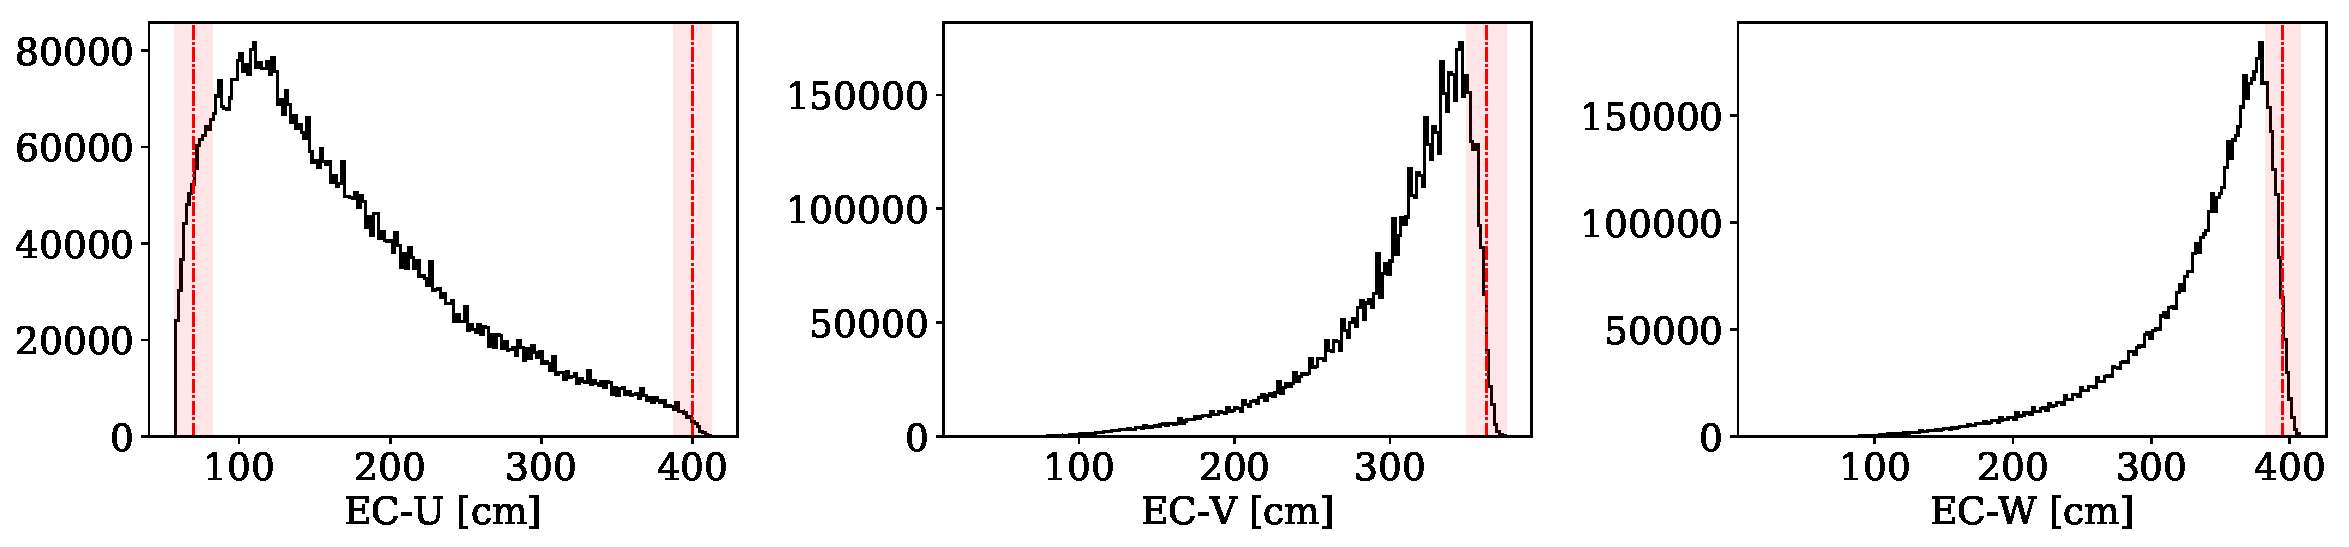
\includegraphics[width=\textwidth]{image/plots/kaon-bsa/ec-fid-sys.pdf}
		\caption{Boundaries and associated uncertainties for the $EC$ coordinate cuts.}
	\end{center}
\end{figure}

The electron identification cuts used on ECAL are varied in order to estimate the dependence of the asymmetry on these parameters.  These boundaries (which are sometimes excluded from systematic uncertainties) produce some of the largest changes in our analysis, associated with the large deviation of the distributions around the cut \ref{fig:ec_fid_sys}.  The shift in the measured beam spin asymmetry is large particularly for low $x$, low $Q^2$, low $P_T$ and high $z$.  These shifts likely arise from the reduction of statistics in the low angle region ($x$ is correlated with $ECU$ with coefficient 0.49, $Q^2$ is correlated with $ECU$ with coefficient 0.8).   

\begin{sidewaysfigure}
	\label{fig:systematic_heatmap_x}
	\begin{center}
		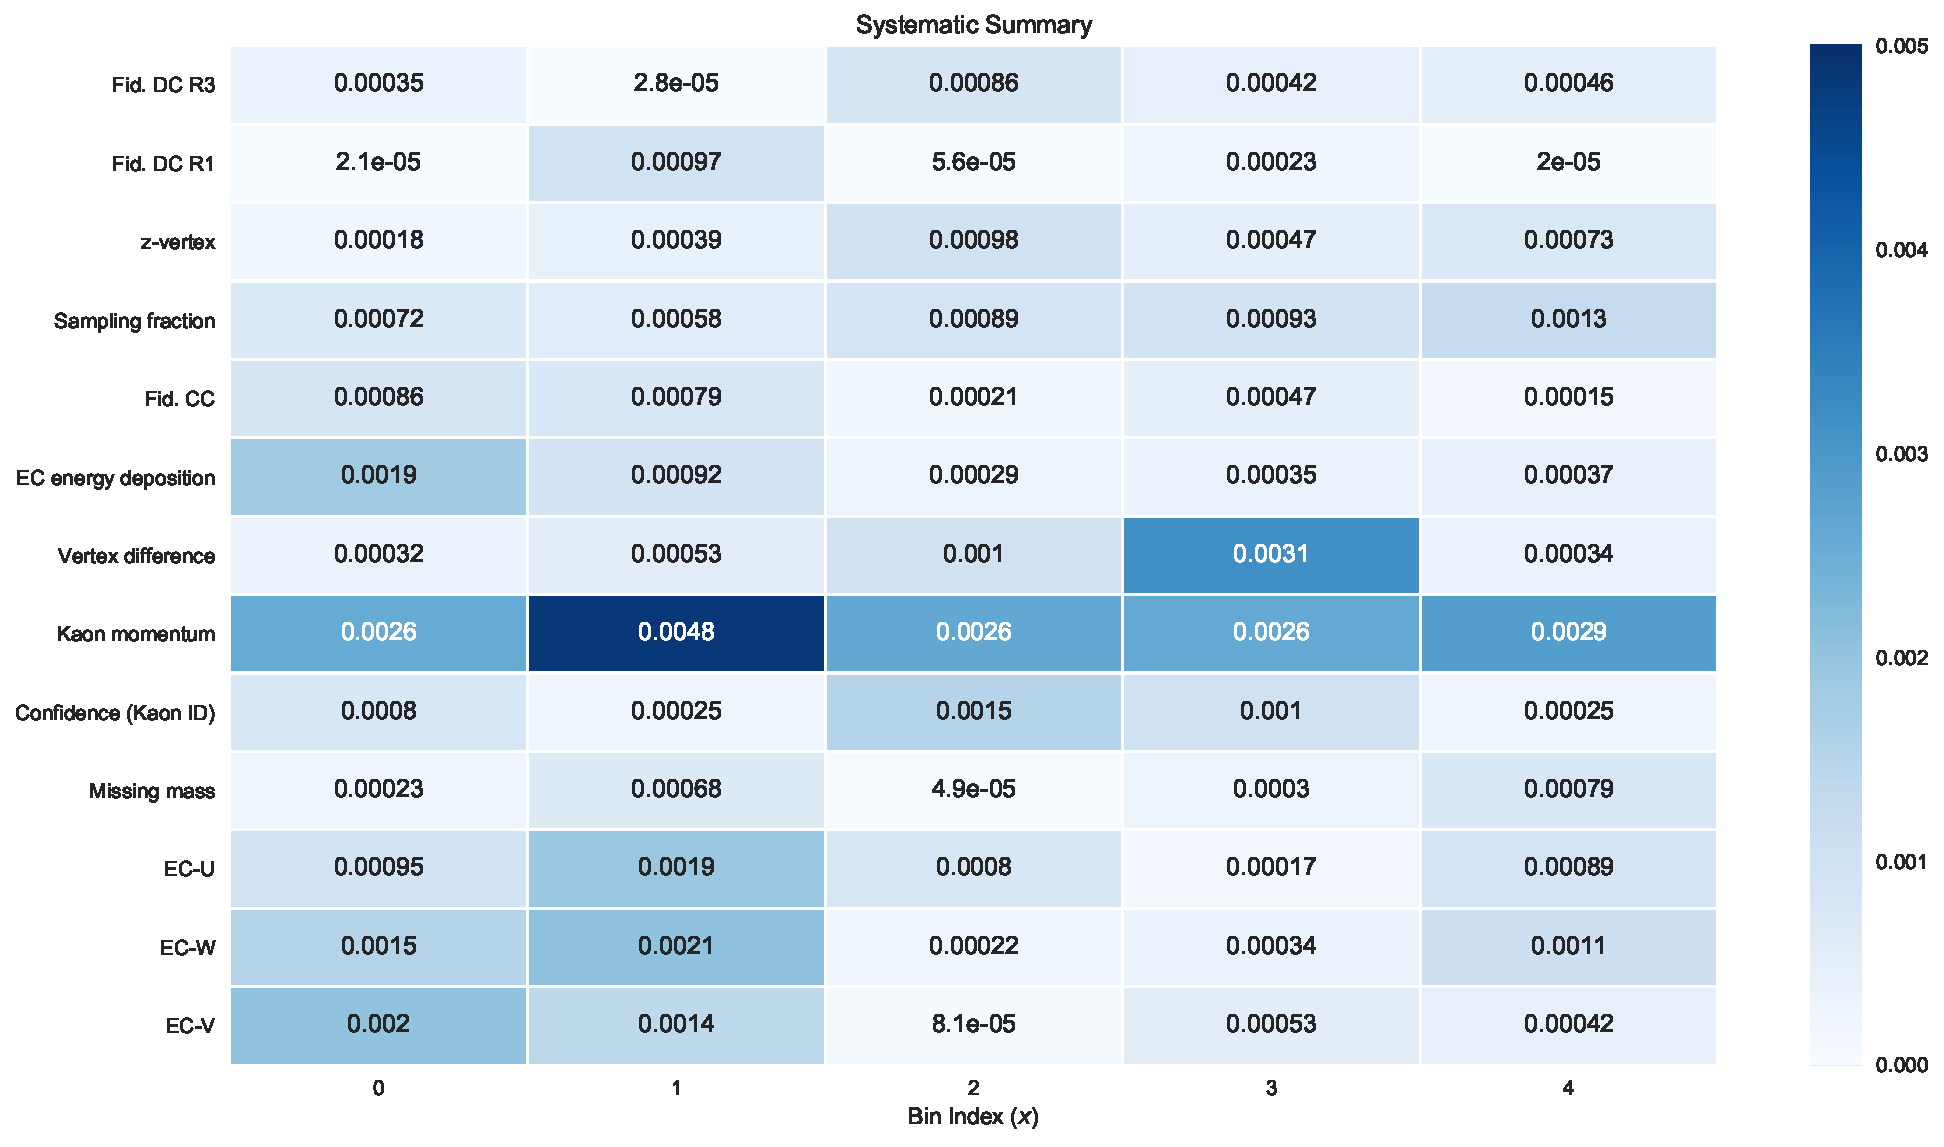
\includegraphics[width=\textwidth]{image/plots/kaon-bsa/systematics_integrated_heatmap_x.pdf}
		\caption{The magnitude of each systematic error source considered is shown above in a heat-map for the $x$ axis.  The vertical scale maximum corresponds to half of a percent.}
	\end{center}
\end{sidewaysfigure}

\subsubsection*{Missing Mass}
To investigate the effect of varying our missing mass cut on the analysis we shift it left and right by 50 MeV, which produces little to no effect.  This is demonstrated in the figures \ref{fig:systematic_heatmap_x} \ref{fig:systematic_heatmap_pt} \ref{fig:systematic_heatmap_z}.  

\subsubsection*{Confidence Level}
The minimum acceptable confidence level is varied between 0.5 at the loosest and 0.6 at the tightest.  For the $x$, $Q^2$, and $P_T$ axes the observed shift is roughly constant regardless of the kinematic bin.  

\begin{sidewaysfigure}
	\label{fig:systematic_heatmap_pt}
	\begin{center}
		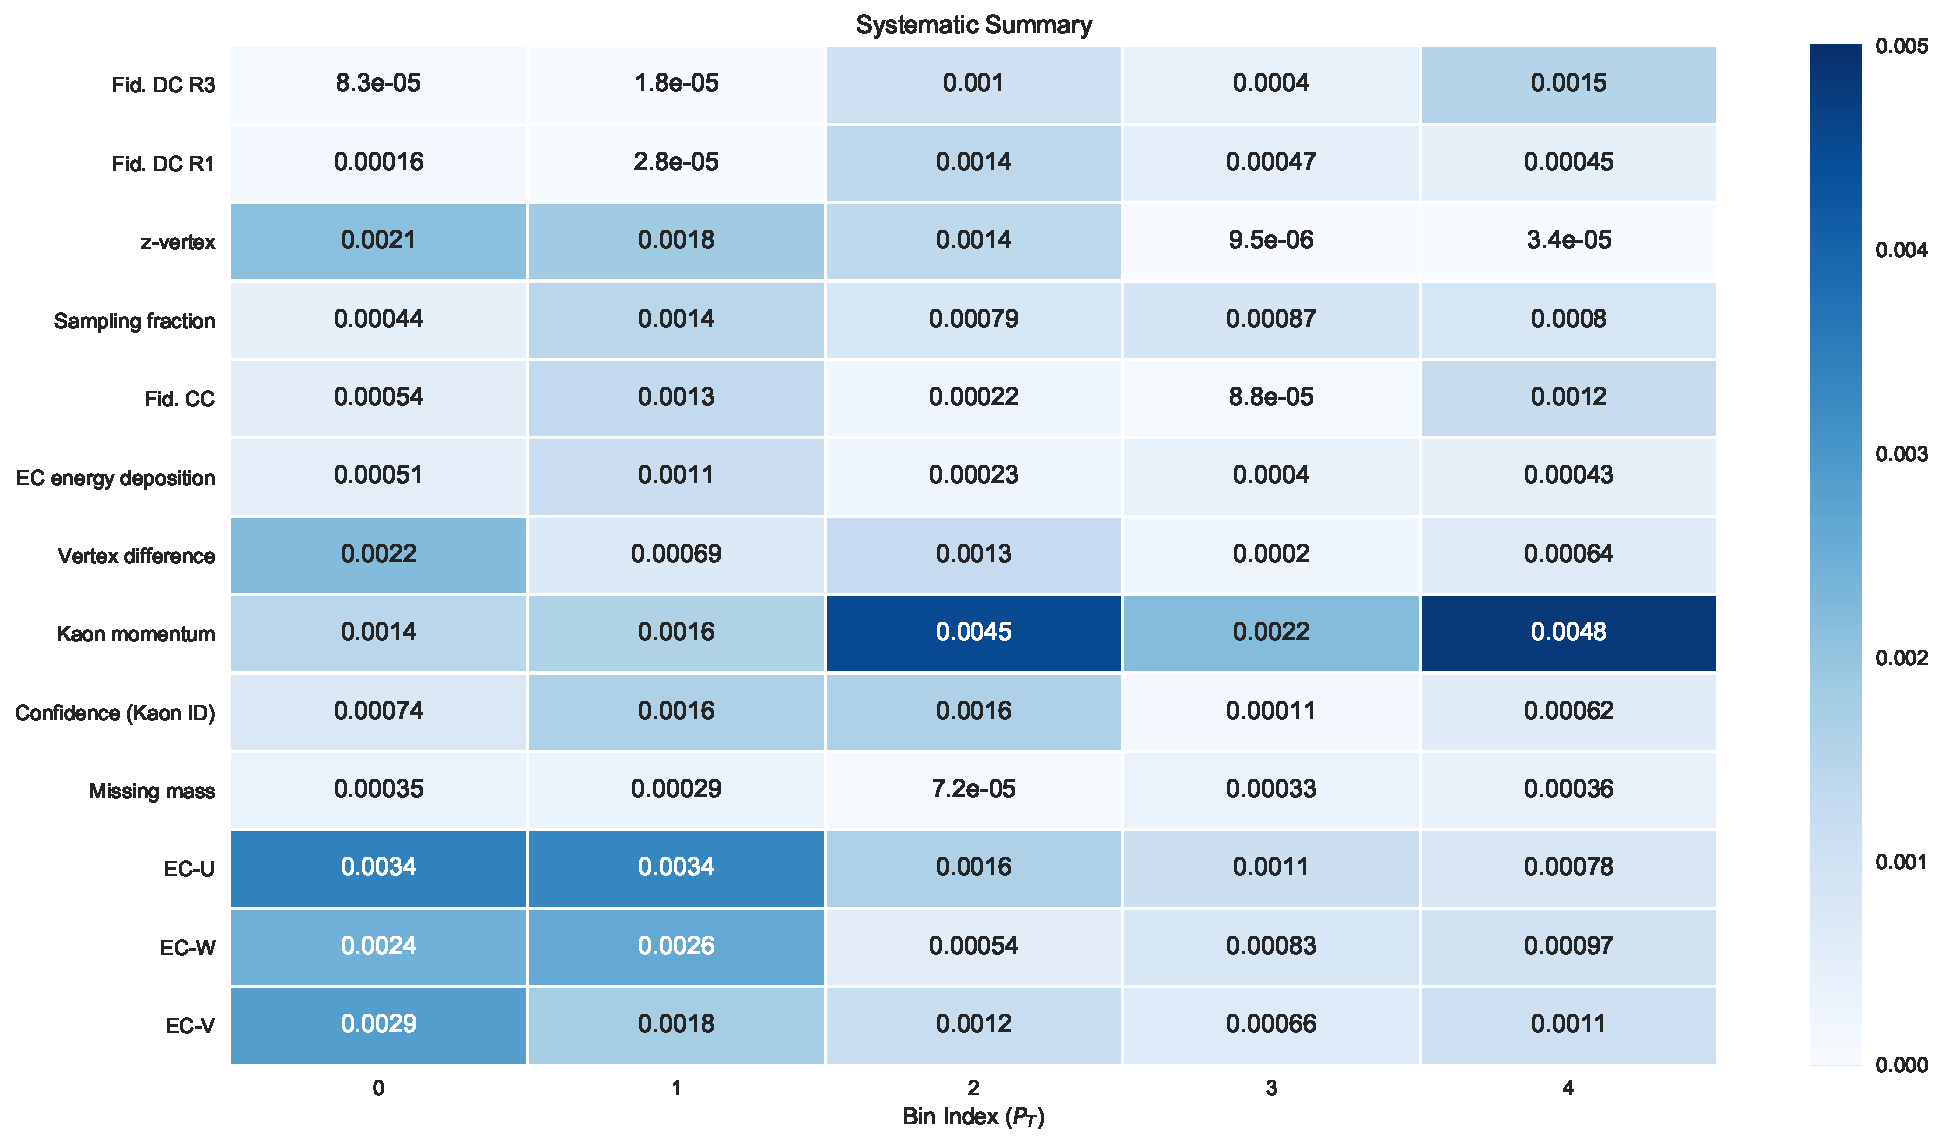
\includegraphics[width=\textwidth]{image/plots/kaon-bsa/systematics_integrated_heatmap_pt.pdf}
		\caption{The magnitude of each systematic error source considered is shown above in a heat-map for the $P_T$ axis.  The vertical scale maximum corresponds to half of a percent.}
	\end{center}
\end{sidewaysfigure}

\begin{sidewaysfigure}
	\label{fig:systematic_heatmap_z}
	\begin{center}
		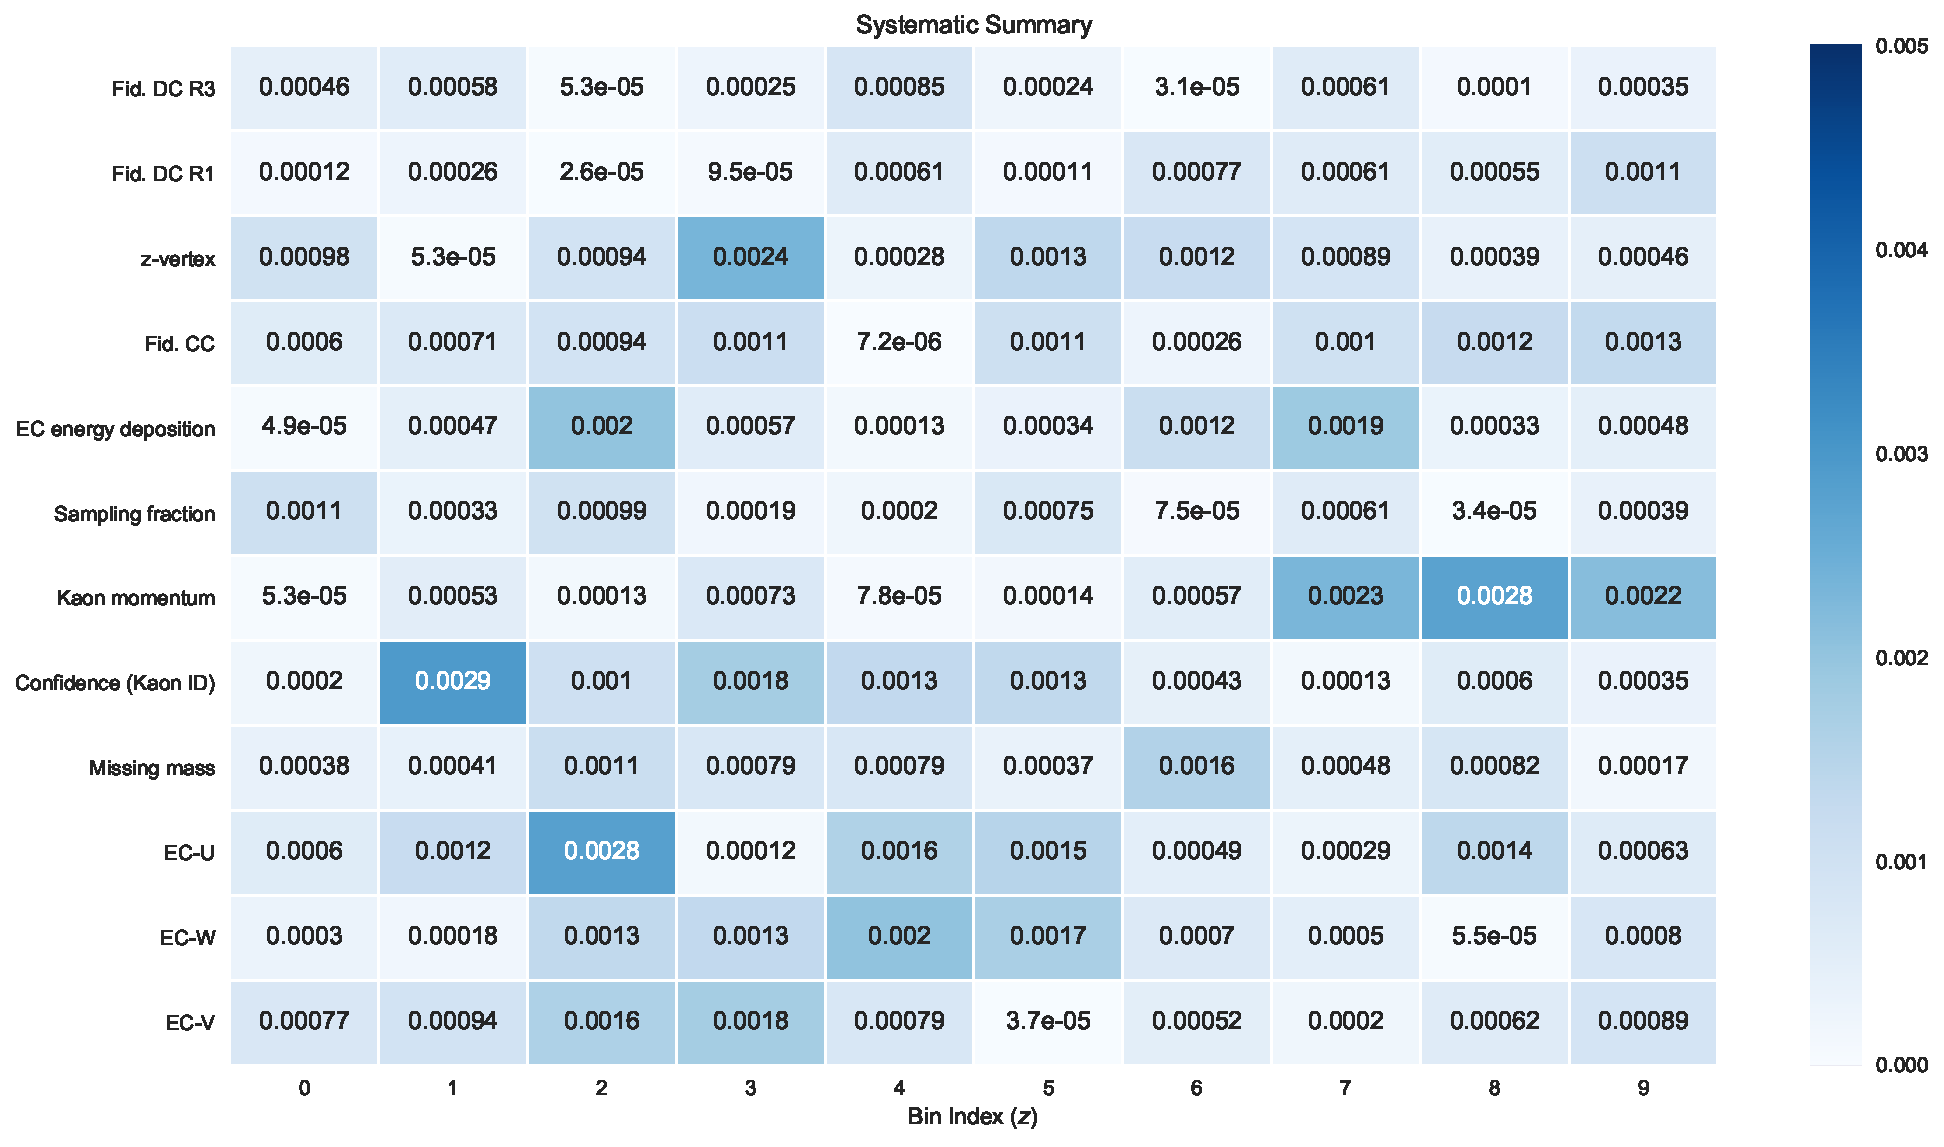
\includegraphics[width=\textwidth]{image/plots/kaon-bsa/systematics_integrated_heatmap_z.pdf}
		\caption{The magnitude of each systematic error source considered is shown above in a heat-map for the $z$ axis.  The vertical scale maximum corresponds to half of a percent.}
	\end{center}
\end{sidewaysfigure}

\subsubsection*{Kaon Momentum}
Monte Carlo analysis of kaon identification purity and efficiency was used to establish a maximum acceptable momentum for kaons included in our analysis.  In order to study the impact of that value (2.0), the value is varied by 100 MeV and the result is included as a systematic error.  

\begin{figure}
	\centering
	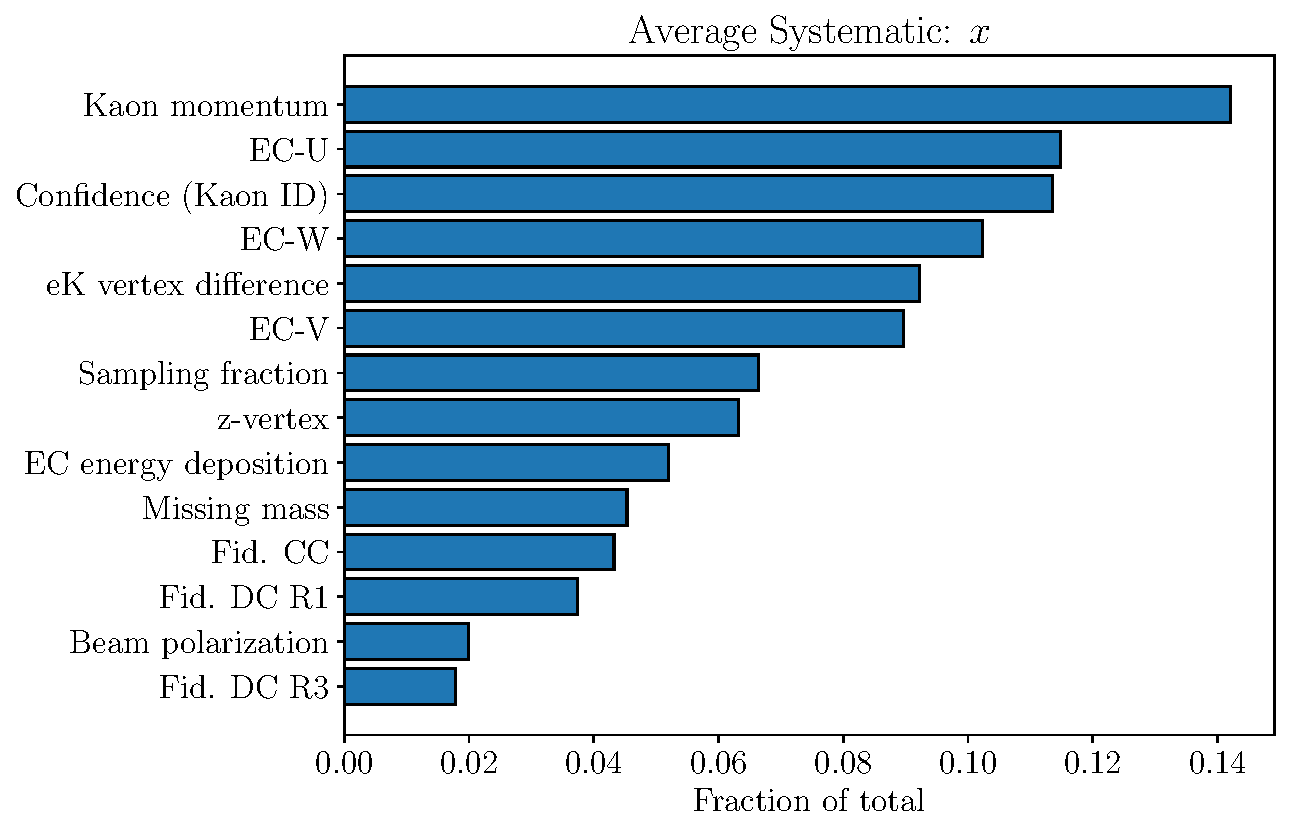
\includegraphics[width=16cm]{image/plots/kaon-bsa/bar-systematics-x.pdf}
	\caption{The relative contribution of each systematic uncertainty to the total is shown above averaged over the bins of the $x$ axis.}
\end{figure}

\begin{figure}
	\centering
	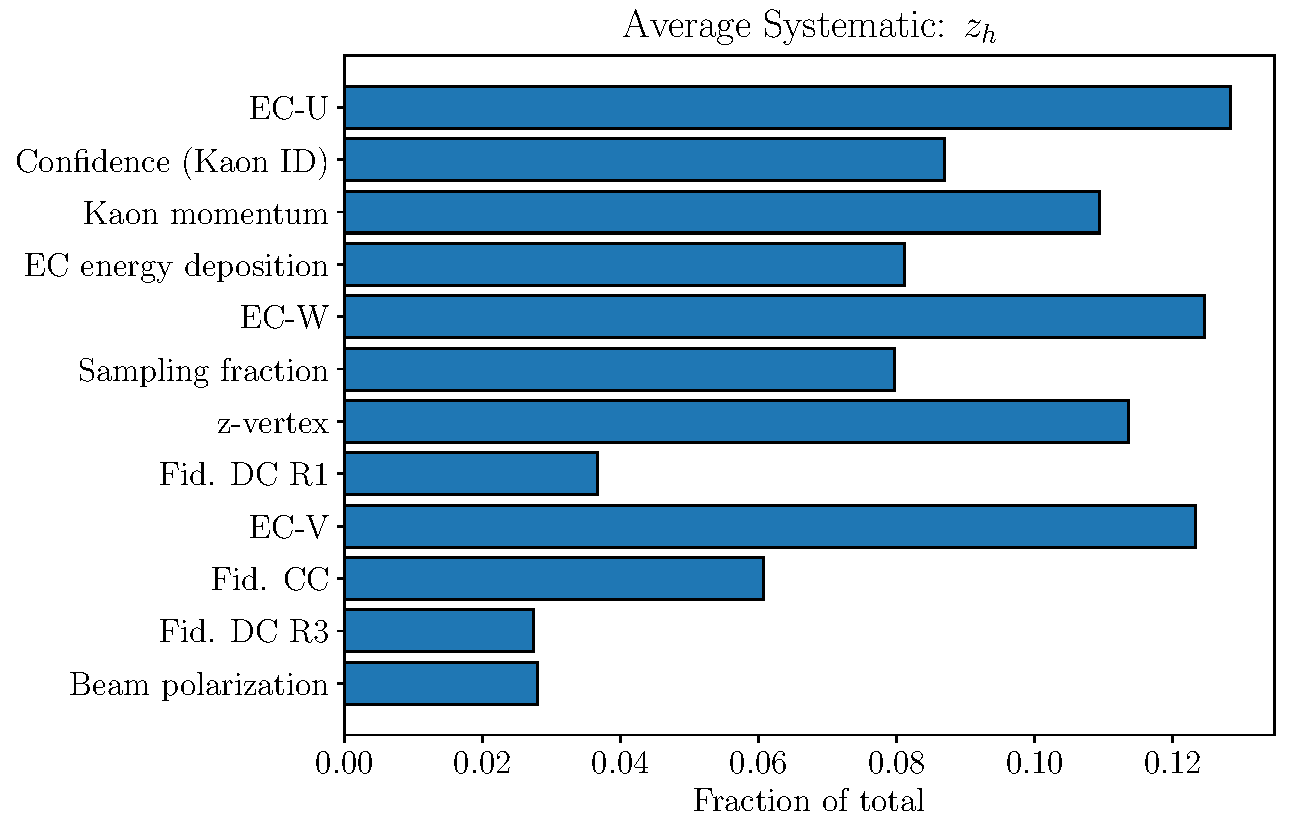
\includegraphics[width=16cm]{image/plots/kaon-bsa/bar-systematics-z.pdf}
	\caption{The relative contribution of each systematic uncertainty to the total is shown above averaged over the bins of the $z$ axis.}
\end{figure}

\subsubsection*{Electromagnetic Calorimeter Energy Cuts}
The momentum dependent sampling fraction cut, as well as the energy deposition cut placed on the inner electromagnetic calorimeter do not contribute much to the total systematic uncertainty.  In this study, the variation of the energy deposited cut by 10 MeV did not have a strong impact on the result.  Additionally, the observed shift was mostly constant over the kinematic variables.  The same is true for the sampling fraction cut.

\subsubsection*{Fiducial Cuts on DC and CC}
The variation of our fiducial cuts on the drift chambers regions 1 and 3, as well as the Cherenkov counter produced no major shift in our measured asymmetries.  This reflects the redundancy of using several fiducial cuts.

\subsubsection*{Vertex Cuts}
The vertex cut position was varied by $\pm 0.5 \; (cm)$ and small changes were observed in the extracted beam spin asymmetries.  Additionally, no kinematic dependence was observed in the shifts.

\section{Extraction of Modulations}

\begin{equation}
	\centering
	\label{fig:replicas-x}
	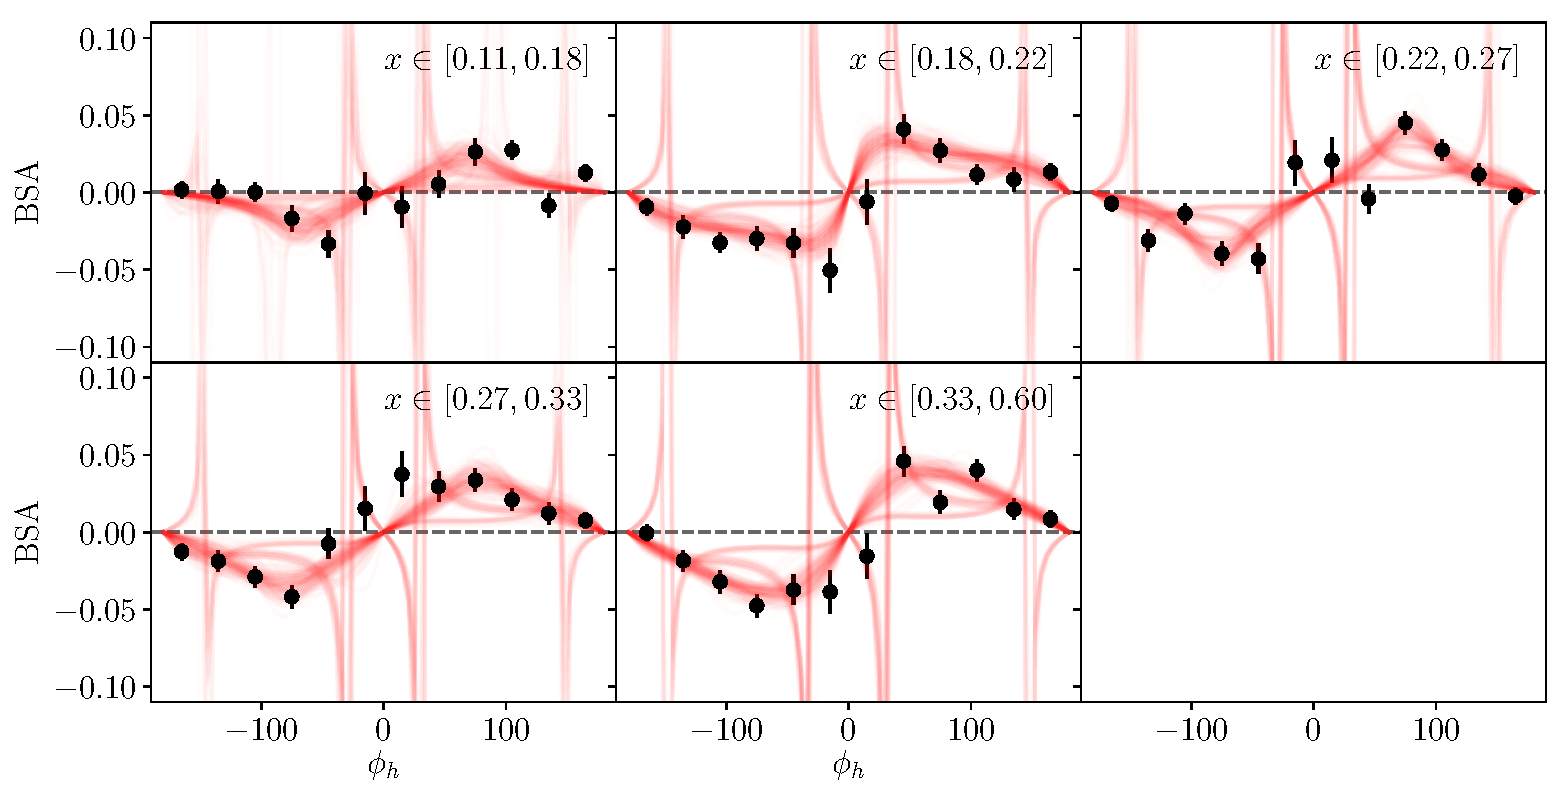
\includegraphics[width=\textwidth]{image/plots/kaon-bsa/grid_bsa_reps_x.pdf}
	\caption{The $\phi_h$ dependence is shown for each bin of $x$, increasing in value from the top left to the bottom right.  The statistical uncertainty is shown as black error bars on each point.  Fits to 256 replicas have been superimposed on the figure.}
\end{equation}

\begin{equation}
	\centering
	\label{fig:replicas-z}
	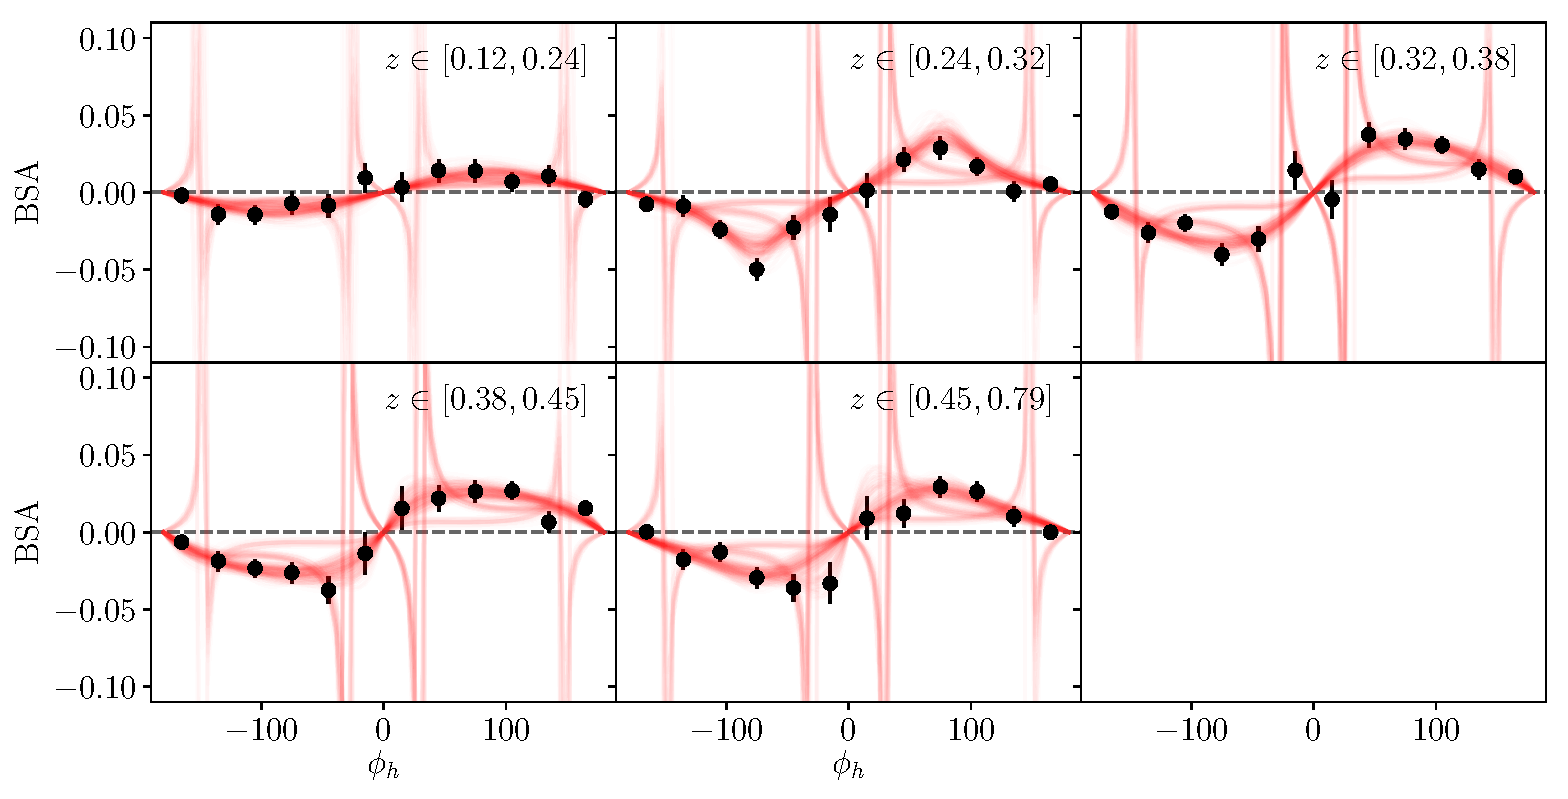
\includegraphics[width=\textwidth]{image/plots/kaon-bsa/grid_bsa_reps_z.pdf}
	\caption{The $\phi_h$ dependence is shown for each bin of $z$, increasing in value from the top left to the bottom right.  The statistical uncertainty is shown as black error bars on each point.  Fits to 256 replicas have been superimposed on the figure.}
\end{equation}

The motivation to measure the beam spin asymmetry in several kinematic bins as well as bins of $\phi_{h}$ is to perform an estimate of the value of structure functions at the kinematic points (more precisely the average value of the structure functions over the range of values included in a point).  To do this, the authors perform parameter estimation on the $\phi_{h}$ distributions taking as a model the theoretical dependence of the beam spin asymmetry on $\phi_{h}$.

\begin{equation}
  f(\phi_h, \vec{a}) = \frac{a_0 \sin\phi_h}{1 + a_1 \cos\phi_h + a_2 \cos(2\phi_h)}
\end{equation}

The parameters $\vec{a}$ are the structure function ratios to be extracted.  The simplest way to extract these parameters is to use $\chi^2$ minimization implemented in a standard fitting package.  In these approaches, $\chi^2$ is defined as the square difference between the observed data values and those predicted by the model, normalized by the error.  If the fluctuation between the data and theory predictions is on the order of the error, the $\chi^2$ is simply on the order of the number of data points.  The parameters $\vec{a}$ which best describe the data are those which make the $\chi^2 (\vec{a})$ assume its minimum value.  This minimization is done in practice with gradient descent or quasi-Newtons method based algorithms like those provided in \texttt{Minuit} or \texttt{scipy.optimize.minimize}, the details of such algorithms will not be discussed here.  It is sufficient to say that these minimization methods produce the parameters $\vec{a}$, and an estimate of the covariance matrix $V$.  The parameters and their errors become the extracted value and uncertainty of the structure function ratio in each bin. \\

Unfortunately, applying the standard single-fit procedure described above does not always produce stable results.  In some cases, the resulting parameter sets are reasonable, in other cases however the parameters in the denominator become nonphysically large and oppose each other.  This effect has motivated previous analysts to search for other means of extracting the dominant $\sin\phi_h$ behavior from the distributions.  One common technique is to assume that the coefficients $a_1$ and $a_2$ of above are small compared to 1.  The analyst can then fit the $\phi_h$ distribution with just one linear parameter $a_0$.  This produces a stable result, but has the disadvantage that one needs to introduce a systematic uncertainty associated with the difference observed between using the full model (with a restricted range for the parameters in the denominator) and the results obtained using the single parameter model.  Additionally, the structure function decomposition of the SIDIS cross section relies on theoretically solid ground, therefore it should be used in its full form.  If the data contain little information regarding the structure function ratios in the denominator, the authors believe it more valuable to demonstrate this by extracting those parameters with (large) errors, rather than ignore their contribution.  In order to accomplish this, the method of replicas (or parametric bootstrapping) is used to perform the parameter estimation.  The replica method consists of generating $N_{rep}$ pseudo-data $\phi_h$ distributions which have a normal distrubition located at the observed value, and with a variance equal to the statistical errors on the associated data point.  

\begin{equation}
  \vec{A}_{rep} = \mathcal{N}(\vec{A}, \vec{\sigma_{A}})
\end{equation}

Here $\vec{A}$ is a vector of length $n_{phi}$ bins, representing the measured beam spin asymmetry for each value of $\phi_h$ in a given kinematic bin.  Each of these distributions is fit with the full model, and the resulting parameter values are saved.  The final reported value for each fit parameter, as well as its uncertainty can be reported as the mean, and standard deviation of the fit results.  This procedure which is similar to bootstrapping, can be seen as an attempt to fit the underlying distribution that generated the data while avoiding the statistical noise.  This technique has been discussed in \cite{computing-watt:2012}.

\begin{gather}
  \expval{a_j} = \sum_{i=1}^{N_{rep}} a_{j}^{(i)} \\
  \sigma_{a_j}^{2} = \frac{1}{N_{rep}-1} \sum_{i=1}^{N_{rep}} (a_{j}^{(i)} - \expval{a_j}) 
\end{gather}

\begin{figure}
	\centering
	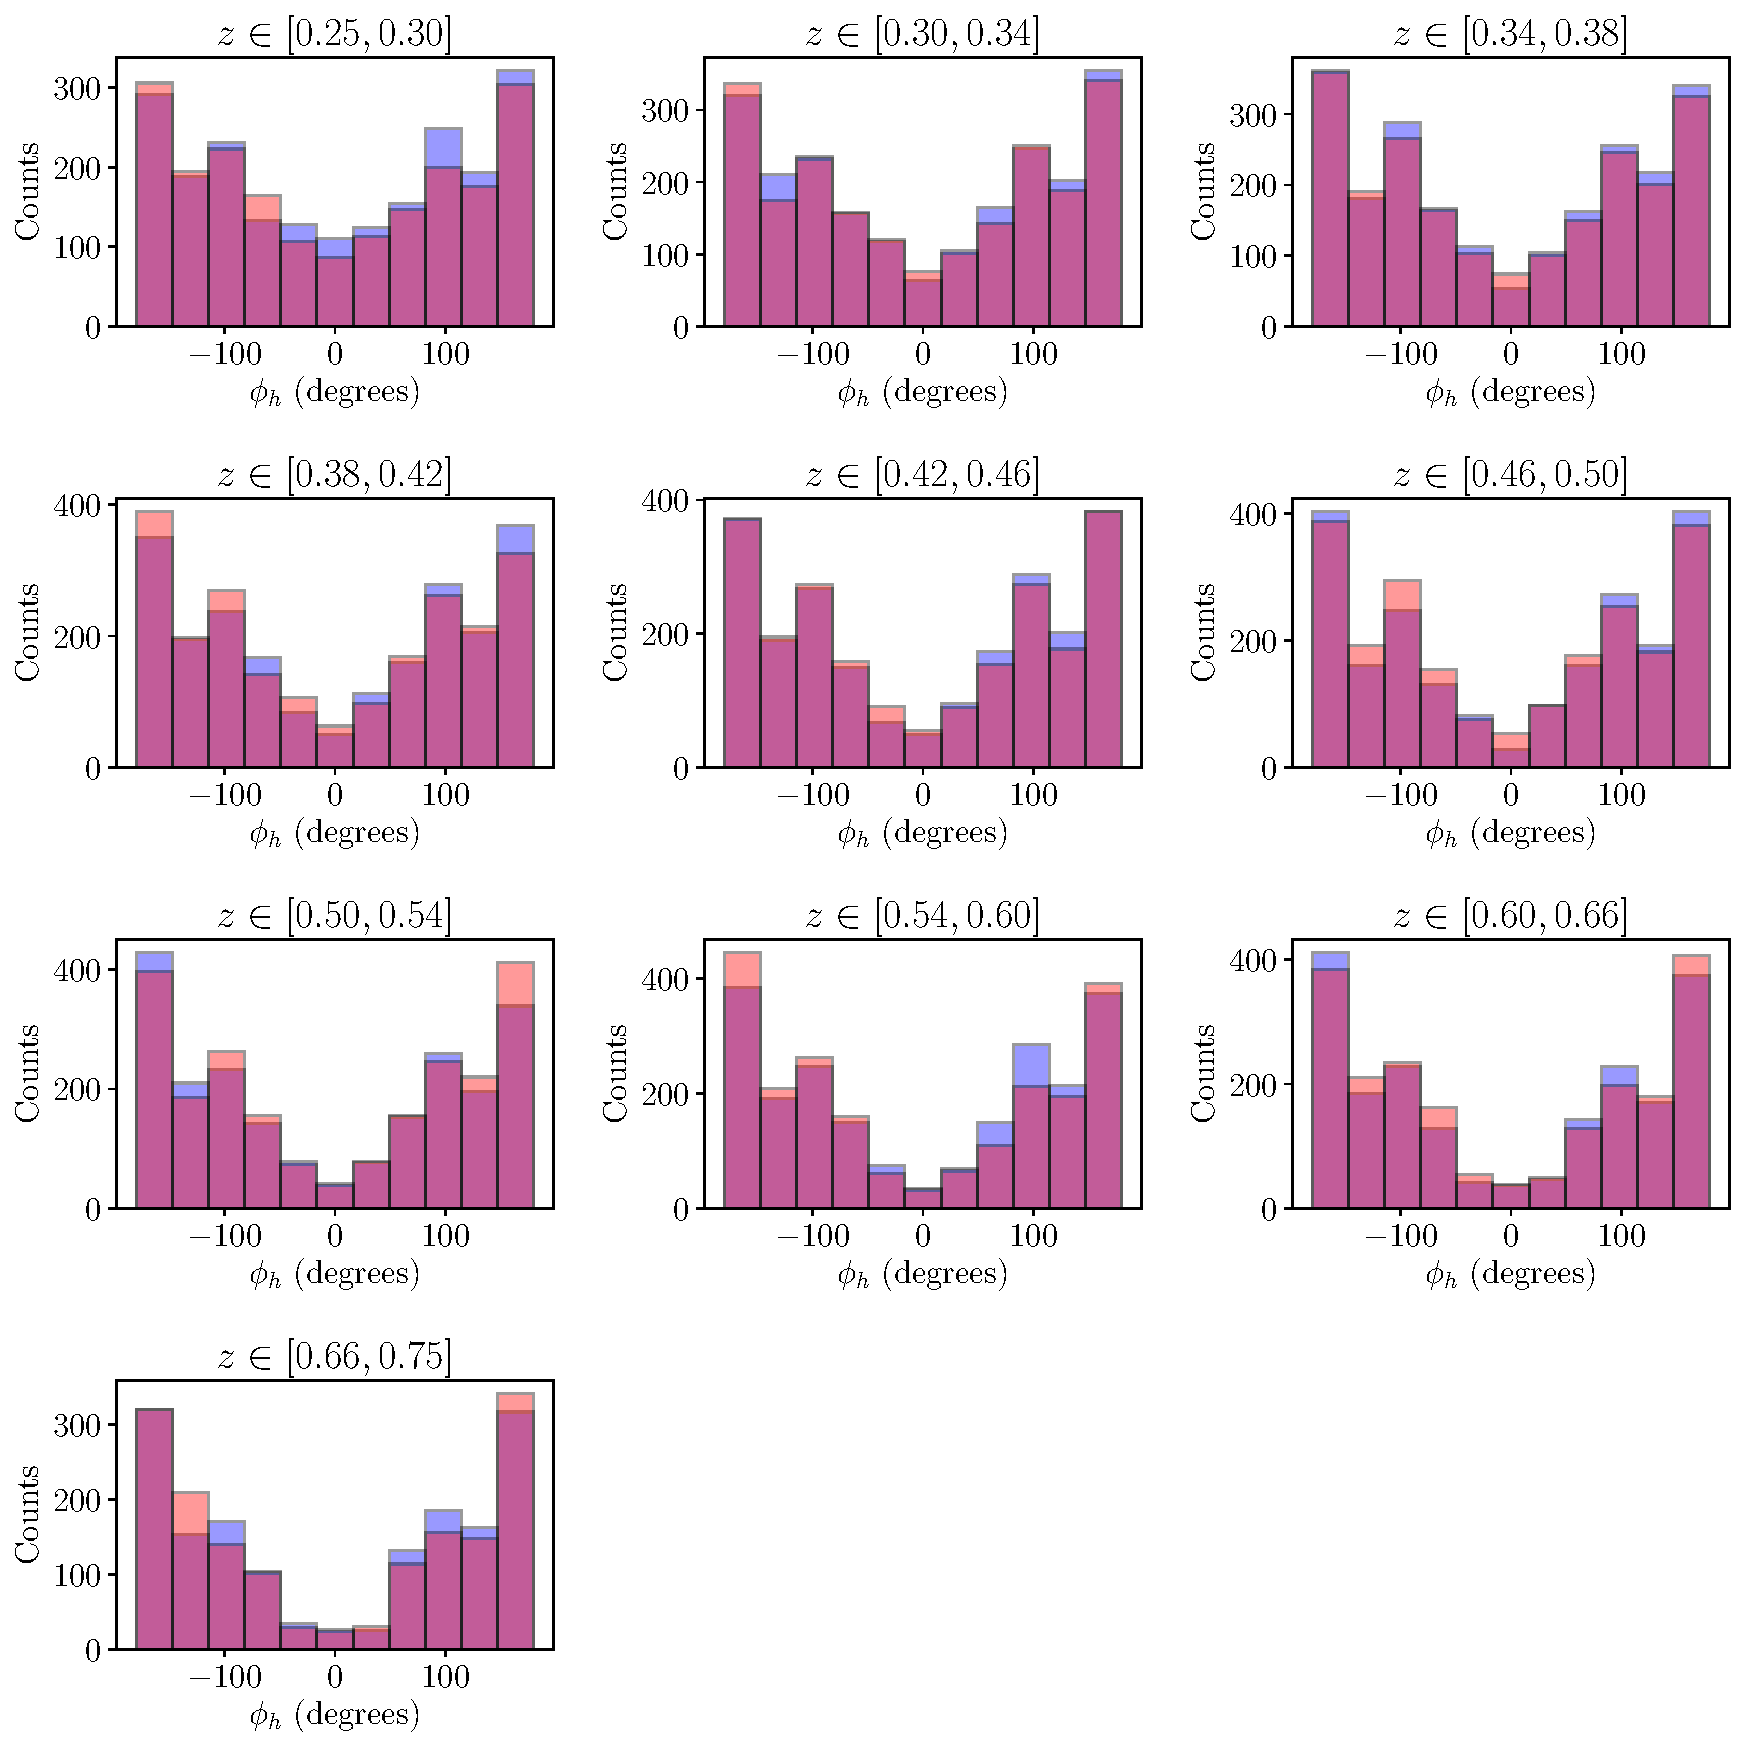
\includegraphics[width=16cm]{image/plots/kaon-bsa/z-phi-counts.pdf}
	\caption{Counts for different helicity states are superimposed for different bins of $z$.}
\end{figure}

\subsubsection*{Results}
%
% This section deserves a more in 
% depth discussion.
%
As is the case for positive pions, the observed structure function ratio $A_{LU}^{\sin\phi}$ is positive for all kinematic points that were measured.  In general, this extraction reveals that the $\sin\phi_h$ moment has a magnitude around 3\% for most kinematic points, and depends weakly on the kinematic variables used in this analysis.  The relative asymmetry value to total error ratio is around 1.5\% for most measured points.

\easyFigure{image/plots/kaon-bsa/alu_sin.pdf}{Our extraction of $A_{LU}^{\sin\phi}$ for the kinematic bins described above.  The black error bars represent uncertainty in the extraction of the parameter value.  Red error bars are systematic uncertainties.}

% Compare to results of W. Gohn (x, Q^2)
\begin{figure}
	\centering
	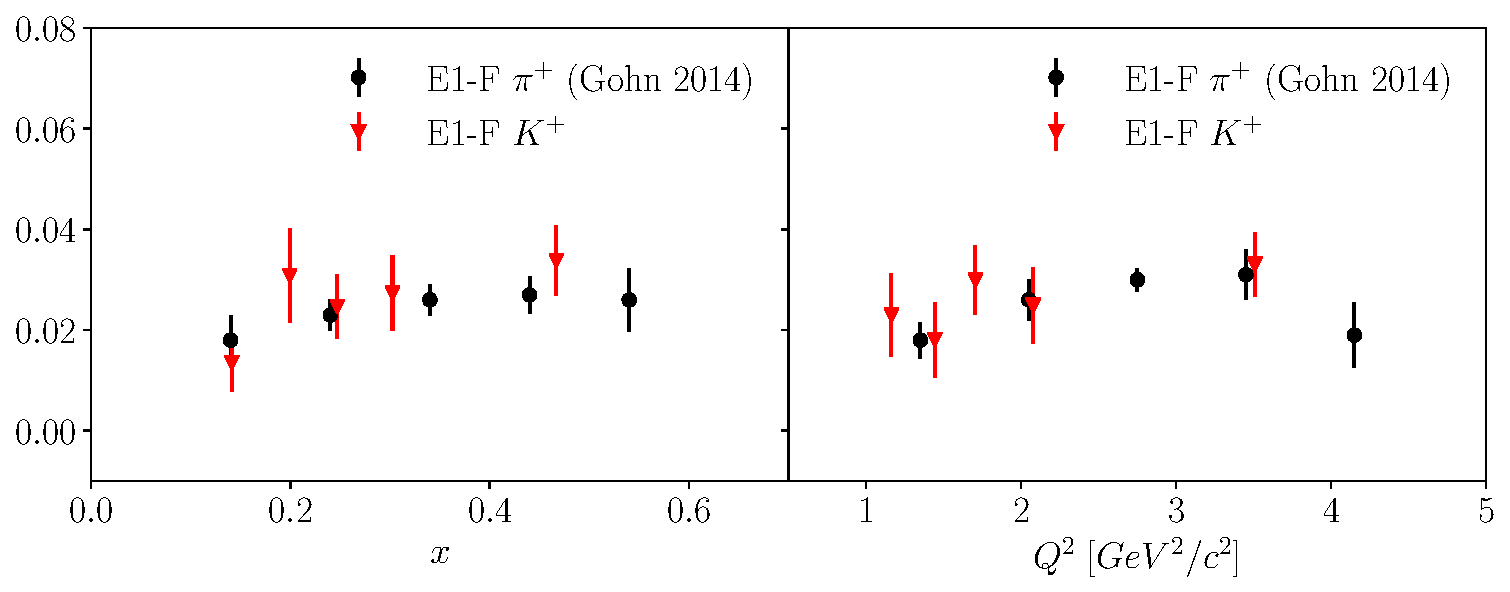
\includegraphics[width=16cm]{image/plots/kaon-bsa/compare-pion-xq2.pdf}
	\caption{In this figure the results of this study for postively charged kaons are compared with previous results from the same dataset produced by \cite{tmds-gohn:2014} for positively charged pions.  This figure shows the $x$ and $Q^2$ dependence of $A_{LU}^{\sin\phi_h}$.}
\end{figure}

% Compare to results of W. Gohn (z, P_T)
\begin{figure}
	\centering
	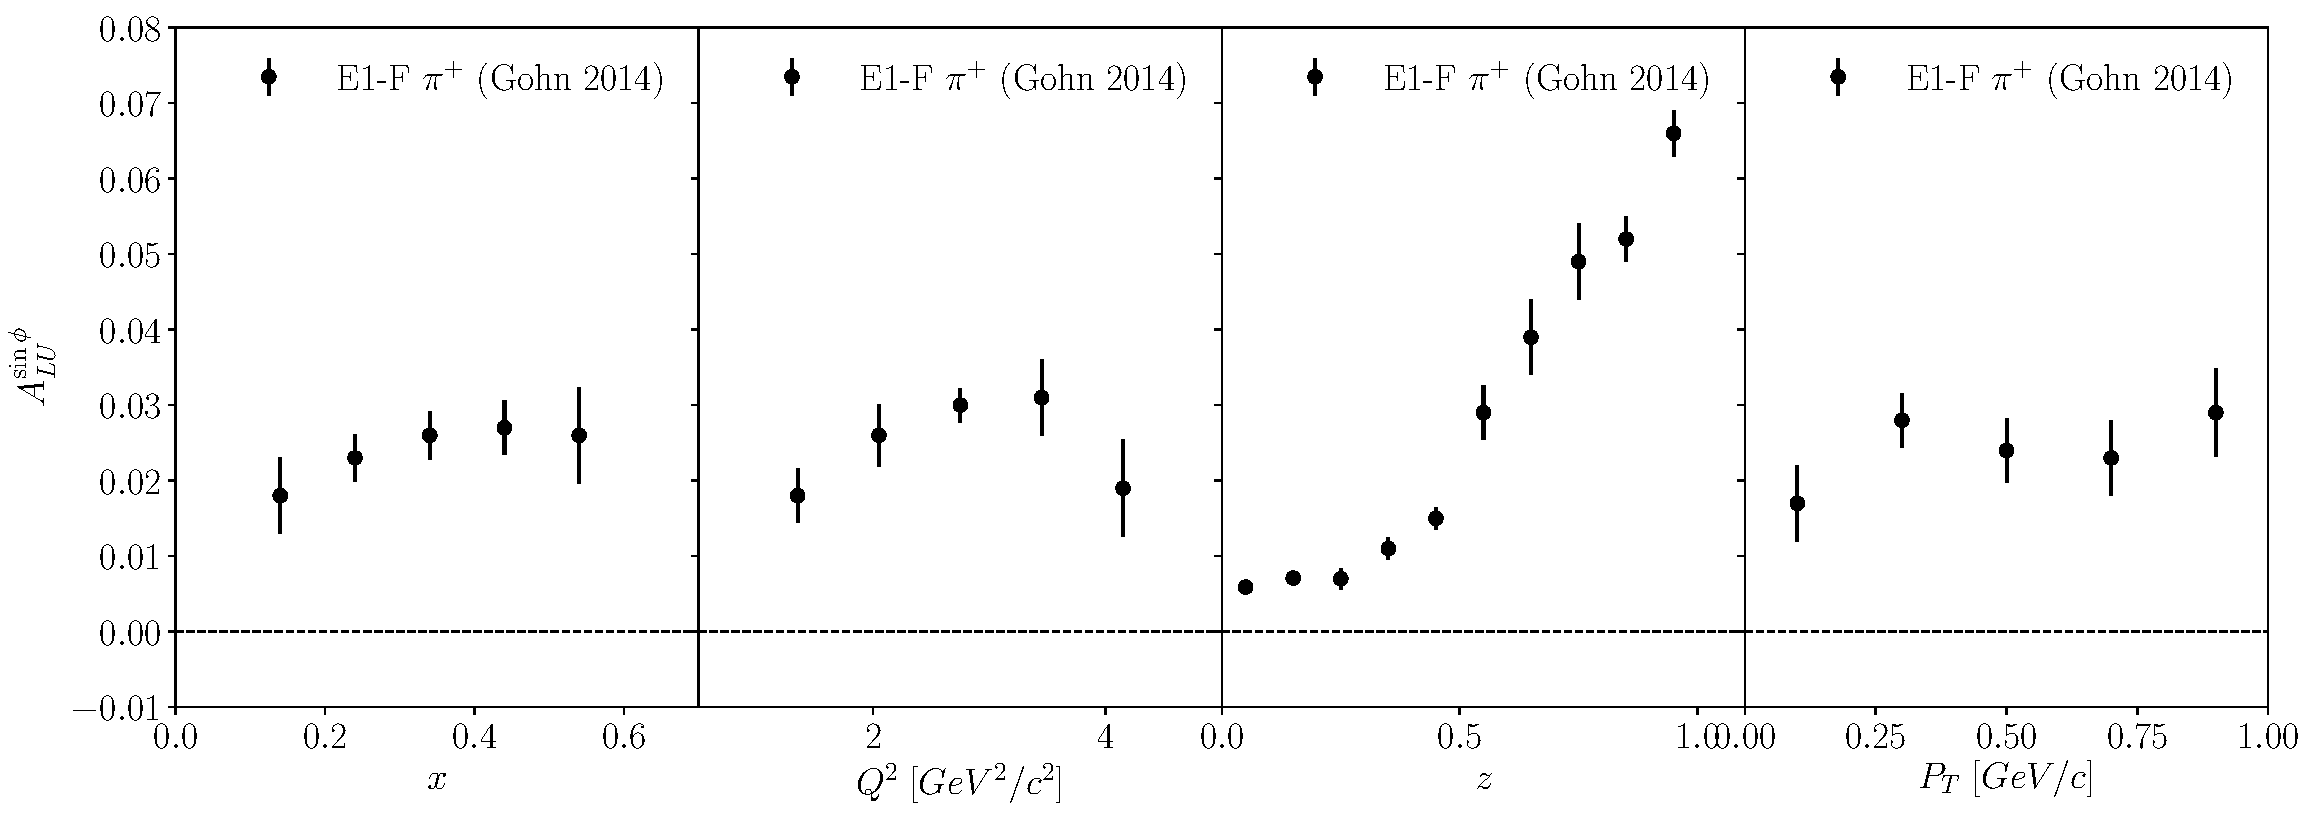
\includegraphics[width=16cm]{image/plots/kaon-bsa/compare-pion-zpt.pdf}
	\caption{In this figure the results of this study for postively charged kaons are compared with previous results from the same dataset produced by \cite{tmds-gohn:2014} for positively charged pions.  This figure shows the $z$ and $P_T$ dependence of $A_{LU}^{\sin\phi_h}$.}
\end{figure}

